\chapter{Conclusion}
%          * Suppositions fondamentales
%          * Adaptations possibles 

\section{Diagramme de GANTT pr�visionnel}

\begin{figure}[H]
  \centering
  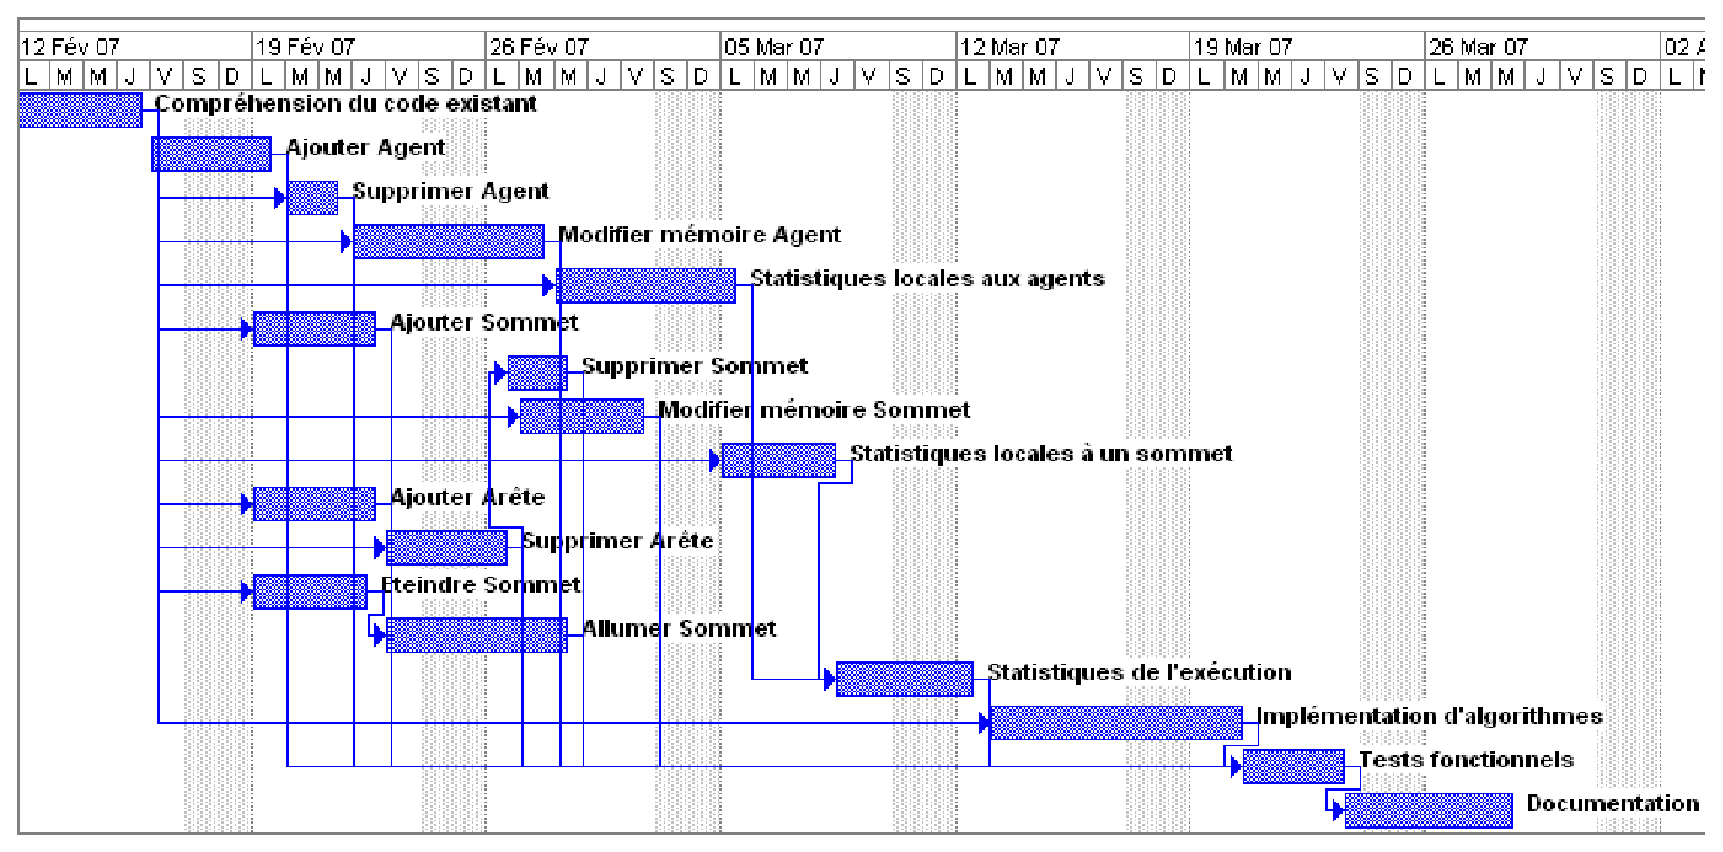
\includegraphics[width=18cm]{img/gantt.eps}
  \caption{Diagramme de Gantt} 
  \label{fig:gantt}
\end{figure}

\section{�volution du syst�me}

Une �volution envisageable de \visidia consisterait � d�velopper un
applet java afin de pouvoir utiliser 
l'application � l'aide d'un simple navigateur internet.

Il pourrait �tre int�ressant �galement de r�aliser de la simulation
d'algorithmes distribu�s sur de vrais r�seaux de machines physiques. 
